\documentclass[letterpaper]{article}
%\usepackage[pass]{geometry}
\usepackage[utf8]{inputenc}
\usepackage{graphicx} % Required for inserting images
%\usepackage[margin=1.1in]{geometry}
\usepackage[bottom]{footmisc}
\usepackage[top = 1in, bottom = 1in, left = 1in, right = 1in]{geometry}
\usepackage{setspace}
%\usepackage{bookman}
\usepackage{amsmath,amssymb}

\usepackage{lscape}
\usepackage{booktabs,caption}
\usepackage{hyperref}
\usepackage[authordate,backend=biber]{biblatex-chicago}
\usepackage[flushleft]{threeparttable}
\hypersetup{
    colorlinks=true,
    linkcolor=blue,
    filecolor=magenta,
    urlcolor=blue,
    pdftitle={Overleaf Example},
    pdfpagemode=FullScreen,
    }
\renewcommand\thefootnote{\textcolor{red}{\arabic{footnote}}}
\renewcommand\thefigure{\textcolor{blue}{\arabic{figure}}}
\renewbibmacro*{cite:labelyear+extrayear}{%
    \iffieldundef{labelyear}
      {}
      {\printtext[bibhyperref]{\textcolor{blue}{\printfield{labelyear}\printfield{extrayear}}}}%
}

\usepackage[edges]{forest}
\usepackage{longtable}
%\usepackage[a6paper,margin=15mm]{geometry}
\usepackage{booktabs}
\usepackage{tabularray}
\usepackage{xcolor}
\usepackage[T1]{fontenc}
\usepackage{babel}
\usepackage{biblatex}
\usepackage{tikz}
\usepackage{changepage}
\usepackage{mathpazo}
\usepackage{subfigure}

\title{Problem Set 6}
\author{Bowei Dong }
\date{}

\begin{document}

\maketitle

\section*{Q3}

Like I mentioned in the last problem set, I have used FEMA county level natural incidents declaration data, to clean this dataset, I have:

\begin{itemize}
    \item Downloaded the dataset from FEMA
    \item Trimmed the data to be 1990-2023
    \item Filtered out non-natural incidents, which include: Fish-loss, human cause, toxic, chemical, biological, terrorists, and others
    \item Reshaped the data set to be a strongly balanced panel, that is, to combine this data with US county list data
\end{itemize}
\section*{Q4}
Please see the visualizations I have created below:
\begin{figure}[h]
  \caption{}
  \label{}
  \centering
    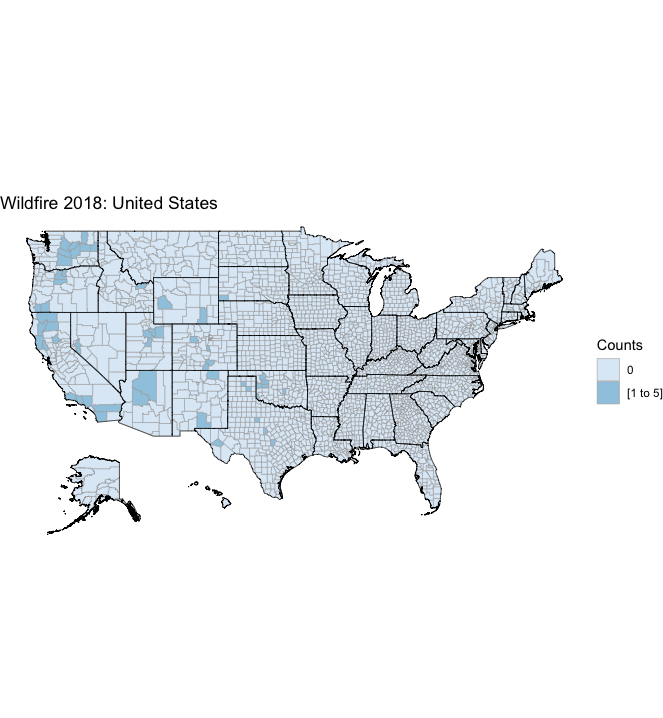
\includegraphics[width=1\textwidth]{PS6a_Dong.png}
\end{figure}

\begin{figure}[h]
  \caption{}
  \label{}
  \centering
    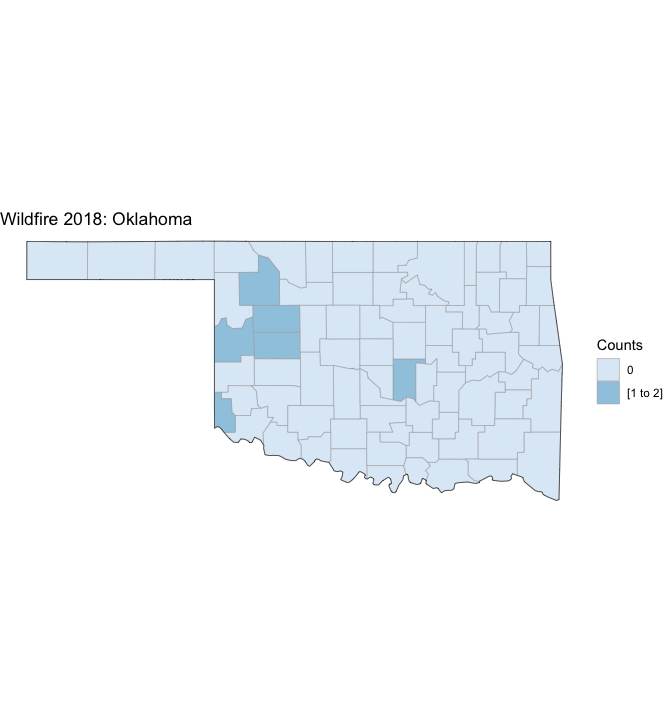
\includegraphics[width=1\textwidth]{PS6b_Dong.png}
\end{figure}

\begin{figure}[h]
  \caption{}
  \label{}
  \centering
    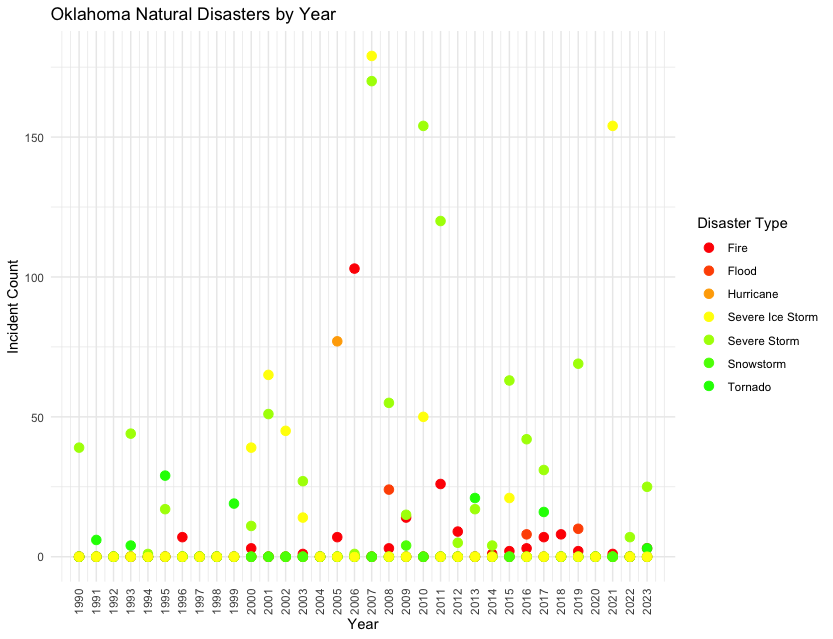
\includegraphics[width=1\textwidth]{PS6c_Dong.png}
\end{figure}

\end{document}
